\subsubsection{}
\label{sec:analysis:research:analogs:telegram}

Одним из самых популярных и быстрорастущих мессенджеров современности является телеграм. 
Сервис разработан братьями Дуровыми и частью бывшей комменды Вконтакте, криптография строится на собственном протоколе MTProto.

На рисунке \ref{sec:analysis:research:analogs:telegram:dialogues} представлен список диалогов в приложении telegram, а на рисунке \ref{sec:analysis:research:analogs:telegram:secretchat} -- пример секретного чата.

\begin{figure}[h]
\centering
\begin{minipage}{.5\textwidth}
  \centering
  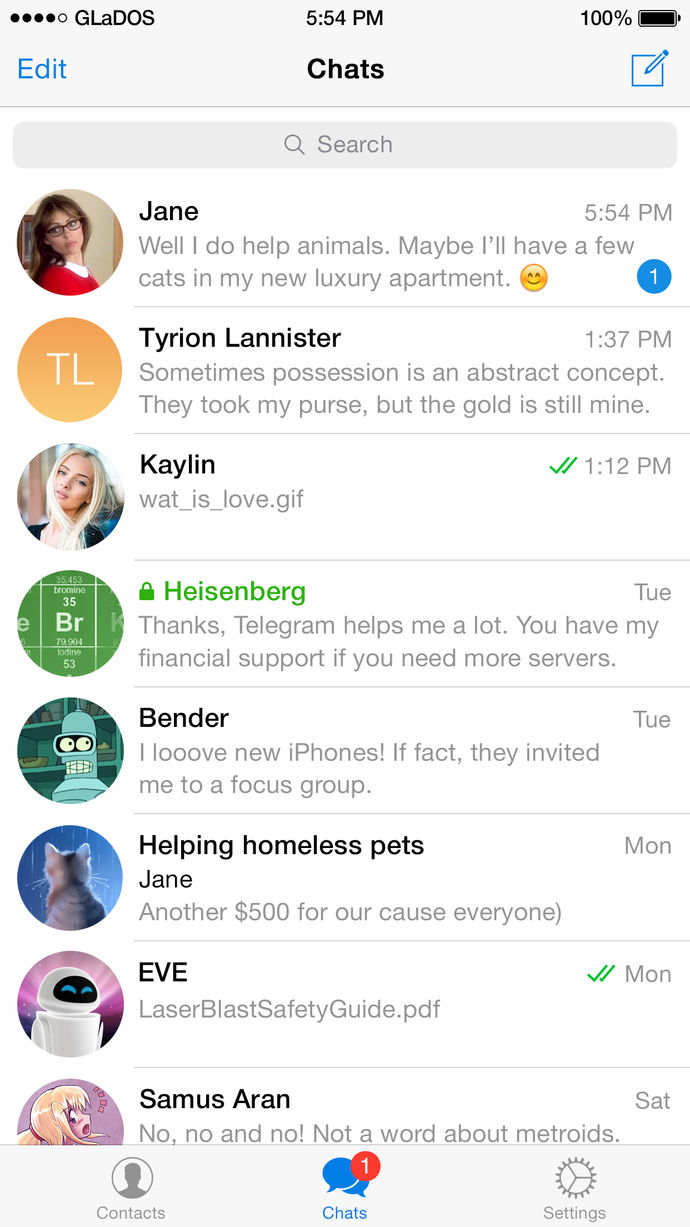
\includegraphics[width=.8\linewidth]{inc/img/tg-dialogues.jpg}
  \captionof{figure}{Список диалогов}
  \label{sec:analysis:research:analogs:telegram:dialogues}
\end{minipage}%
\begin{minipage}{.5\textwidth}
  \centering
  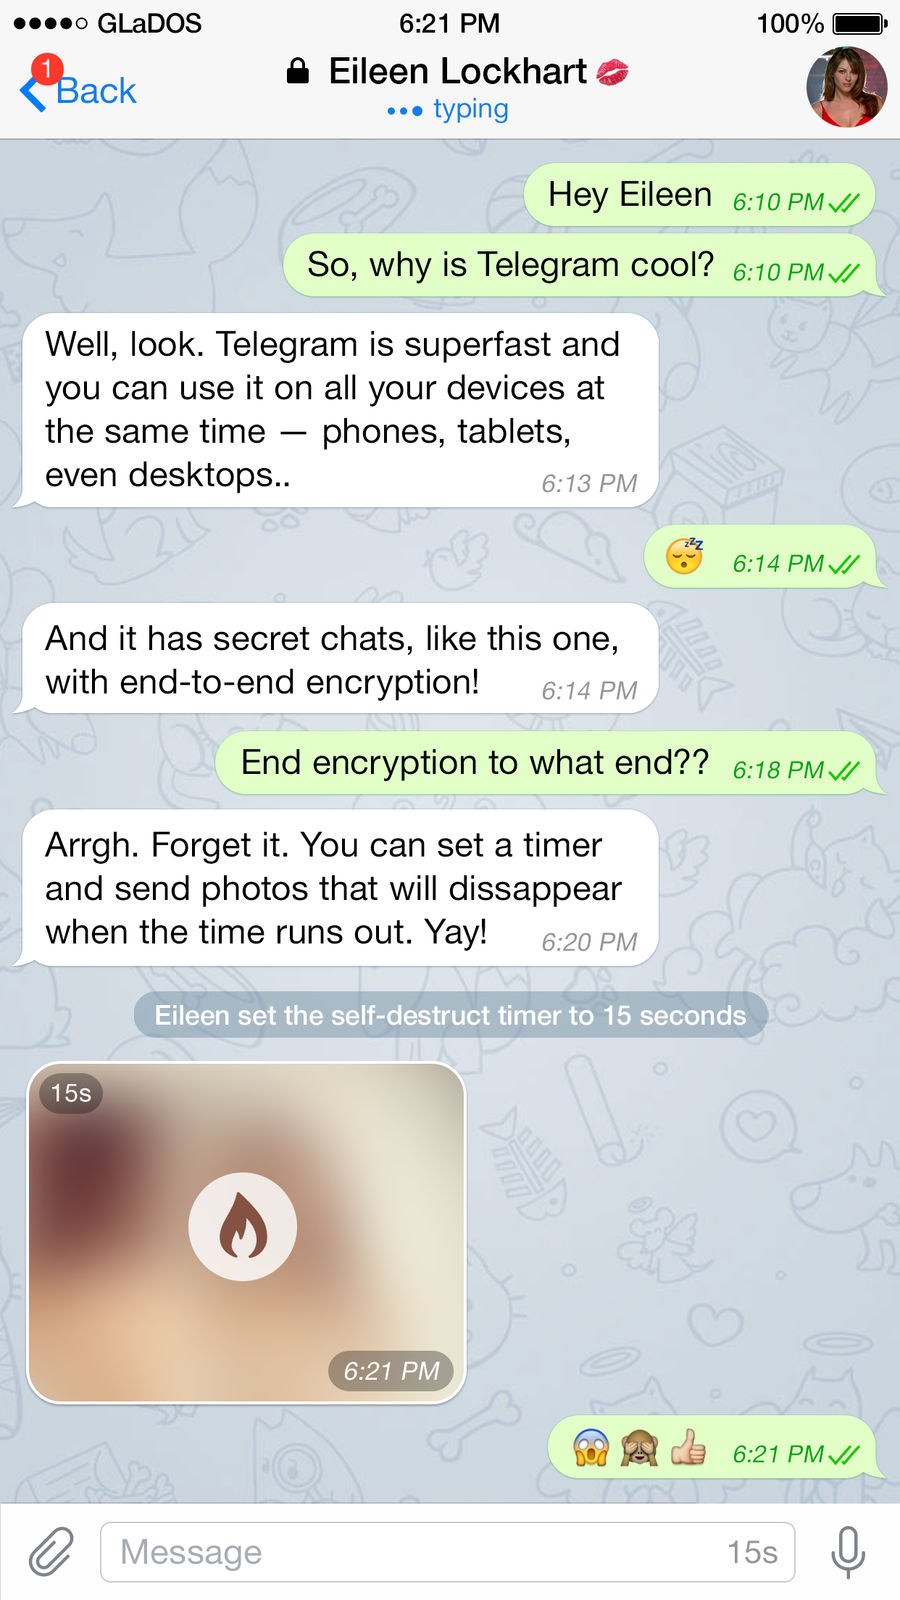
\includegraphics[width=.8\linewidth]{inc/img/tg-secretchat.jpg}
  \captionof{figure}{Секретный чат}
  \label{sec:analysis:research:analogs:telegram:secretchat}
\end{minipage}
\end{figure}

Стоит ближе рассмотреть протокол MTProto и критику, направленую на него. Протокол спроектирован для доступа к серверному \gls{api} из приложений, работающих на мобильных устройствах. 
The protocol is subdivided into three virtually independent components:
Протокол разделён на три виртуально независимые части: 
\begin{itemize}
	\item \textbf{Высокоуровневый компонент(язык запросов)} -- определяет способ, посредством которого запросы и ответы API преобразуются в двоичные сообщения;
	\item \textbf{Уровень криптографии(авторизации)} -- определяет способ шифрования сообщений перед передачей через транспортный протокол;
	\item \textbf{Транспортный компонент} -- определяет метод для клиента и сервера для передачи сообщений по другому существующему сетевому протоколу (например, HTTP, HTTPS, TCP, UDP).
\end{itemize}

На рисунке \ref{sec:analysis:research:analogs:telegram:mtproto1} представлена упрощённая схема взаимодействия клиента и сервера, ипользующих протокол MTProto.

\begin{figure}[h]
  \centering
    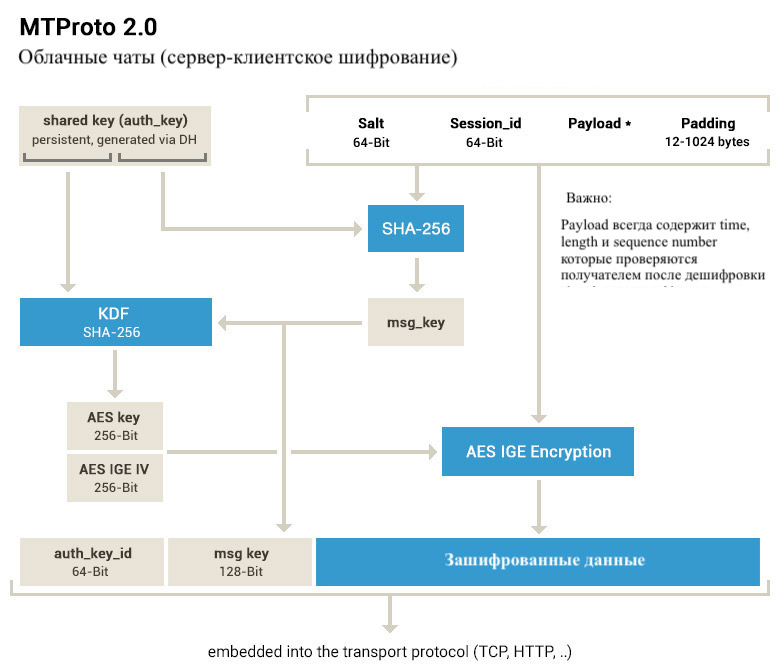
\includegraphics[width=0.8\textwidth]{inc/img/mtproto1.jpeg}
  \caption{Схема общения при помощи MTProto}
  \label{sec:analysis:research:analogs:telegram:mtproto1}
\end{figure}

Перед отправкой сообщения, оно зашифровывается определенным образом, а над ним добавляется \textit{внешний заголовок}, который представляет собой: 64-битный идентификатор ключа (который однозначно идентифицирует ключ авторизации для сервера, а также пользователя) и 128-битный ключ сообщения. Пользовательский ключ вместе с ключом сообщения определяет фактический 256-битный ключ, который шифрует сообщение с использованием шифрования AES-256. Стоит обратить внимание, что начальная часть сообщения, которое должно быть зашифрована, содержит переменные данные (сеанс, идентификатор сообщения, порядковый номер, соль сервера), который, очевидно, влияет на ключ сообщения (и, следовательно, на ключ AES и iv). Ключ сообщения определяется как 128 средних бит SHA256 тела сообщения (включая сеанс, идентификатор сообщения и так далее).

Мессенджер распространяется бесплатно, не поддерживает корпоративные аккаунты и использует собственную облачную архитектуру. Клиентские приложения пишутся сторонними командами, что несколько снижает уверенность в криптографической стойскости всего продукта. Основным нареканием в сторону протокола от криптографических экспертов является его закрытость. Хорошие алгоритмы и протоколы шифрования строятся на математических доказательствах невозможности подобрать ключ шифрования в разумное время и свободно открывают реализацию для публики, позволяя сообществу убедиться в надёжности подхода и помочь найти изъяны имплементации.